\documentclass{article}
\usepackage[T1]{fontenc}
\usepackage[utf8]{inputenc}
\usepackage[portuguese]{babel}

\title{Iniciação Científica\\
Deep Reinforcement Learning}
\author{Lucas Emanuel Resck Domingues\\
Orientador: Dr. Jorge Poco}
\date{July 2020}

\usepackage{natbib}
\usepackage{graphicx}

\begin{document}
    \maketitle

    \tableofcontents

    \section{Introdução}
        % Sigla DRL
        % Cronograma?? 
    
    \section{Estudos}

        Os estudos na área de \textit{Deep Reinforcement Learning}
        começaram na segunda metade de agosto, com a leitura de
        materiais disponibilizados online pelo Instituto de Tecnologia
        de Massachusetts (\textit{MIT})
        % http://introtodeeplearning.com/2019/index.html (como referenciar está na página web)
        , seções 1 e 3 (parte 1 e laboratório). Esses estudos avançaram através dos materiais
        disponibilizados pela Universidade da Califórnia em Berkeley
        % http://rail.eecs.berkeley.edu/deeprlcourse-fa18/
        para as suas aulas de outono de 2018: aulas (\textit{slides} e vídeos) de 1 a 7,
        \textit{homeworks} 1 e 2. Isso até meados do início de novembro.

        As aulas na \textit{UC Berkeley} cobriram conceitos iniciais
        de \textit{Machine Learning}, como \textit{Supervised Learning} e \textit{Imitation
        Learning}, assim como conceitos fundamentais de \textit{Reinforcement Learning},
        como \textit{Q-Functions} e \textit{Value Functions}. A parte "\textit{Deep}"\ também entra
        nesse material, com aulas e \textit{homeworks} fazendo uso de redes neurais
        com a biblioteca \textit{TensorFlow} para \textit{Python}.

        A teoria de redes neurais é relativamente simples, mas a
        implementação não é trivial. Para me acostumar com a execução de códigos
        no meu computador, busquei entender e executar uma implementação de 
        um algoritmo de \textit{Reinforcement Learning} para o jogo \textit{Super
        Mario Bros.}
        % https://medium.com/datadriveninvestor/super-mario-bros-reinforcement-learning-77d6615a805e
        .

        Os \textit{homeworks} por sua vez foram muito interessantes.
        O primeiro deles basicamente se tratava de \textit{Imitation Learning}.
        Dessa forma, pude "ensinar"\ um humanoide (do ambiente virtual \textit{Mujoco}, Figura \ref{fig:humanoid}) a como correr, sem cair,
        apenas copiando um humanoide experiente. O segundo homework tratou de 
        \textit{policy gradients}.

        \begin{figure}[h!]
            \centering
            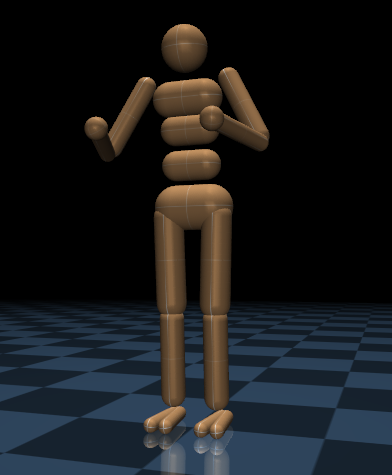
\includegraphics[scale=0.8]{humanoid.png}
            \caption{Humanoide do ambiente virtual \textit{Mujoco}.}
            % http://www.mujoco.org/forum/index.php?attachments/humanoid-png.48/
            \label{fig:humanoid}
        \end{figure}

    \section{Implementações}

        Após estudos introdutórios acerca do tema, decidimos
        que seria interessante aplicá-los, do início de novembro ao início de fevereiro.
        Realizei os exercícios
        disponibilizados pela \textit{UC Berkeley} para \textit{Reinforcement
        Learning}
        % http://ai.berkeley.edu/reinforcement.html
        , sendo que o último deles é a implementação para o jogo
        do \textit{Pac-Man}, buscando "ensinar"\ o personagem para que
        ele vença o jogo sozinho (ver Figura \ref{fig:pac-man}).

        \begin{figure}[h!]
            \centering
            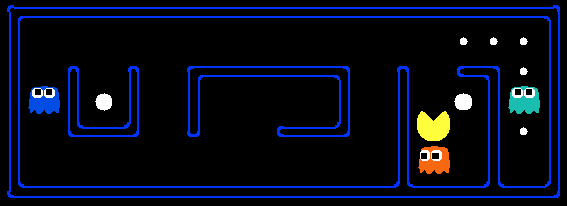
\includegraphics[width=\textwidth]{pac_man.png}
            \caption{Ambiente para o \textit{Pac-Man}.}
            % http://ai.berkeley.edu/projects/release/reinforcement/v1/001/capsule.png
            \label{fig:pac-man}
        \end{figure}

        Foi muito conveniente também a implementação de vários dos 
        algoritmos de \textit{Reinforcement Learning} agregados em
        % https://medium.com/@m.alzantot/deep-reinforcement-learning-demysitifed-episode-2-policy-iteration-value-iteration-and-q-978f9e89ddaa
        , utilizando os ambientes da biblioteca para \textit{Reinforcement Learning} chamada \textit{Gym}.
        Utilizando esses ambientes, como o da Figura \ref{fig:mountaincar-v0}, o objetivo é, em geral, treinar
        o personagem para realizar uma tarefa.
        O algoritmo de \textit{Q-learning} foi um dos algoritmos implementados em
        % https://medium.com/@m.alzantot/deep-reinforcement-learning-demysitifed-episode-2-policy-iteration-value-iteration-and-q-978f9e89ddaa
        .
        A base desse algoritmo é uma tabela,
        utilizada para tentar aproximar uma função. Substituindo essa tabela por
        uma rede neural (para executar uma mesma função), o resultado também fica muito
        legal. Os códigos podem ser conferidos no meu repositório no \textit{GitHub}
        % https://github.com/lucasresck/deep-reinforcement-learning
        .

        \begin{figure}[h!]
            \centering
            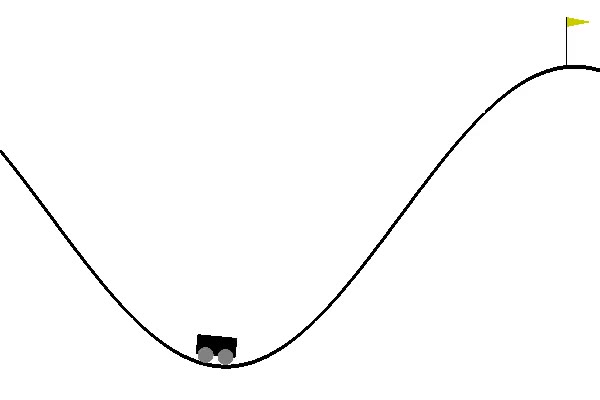
\includegraphics[width=\textwidth]{mountaincar_v0.jpg}
            \caption{Ambiente \textit{MountainCar-v0} da biblioteca \textit{Gym}.
            O objetivo nesse ambiente é fazer o carrinho chegar ao topo da montanha.}
            % https://gym.openai.com/videos/2019-10-21--mqt8Qj1mwo/MountainCar-v0/poster.jpg
            \label{fig:mountaincar-v0}
        \end{figure}

    \section{\textit{Deep Q-Learning}}

        O algoritmo de \textit{Deep Q-Learning} com certeza foi a parte mais desafiadora
        até agora. Esse é um algoritmo que foi publicado por
        % https://arxiv.org/abs/1312.5602
        % https://www.nature.com/articles/nature14236
        e descreve como treinar uma rede neural para aprender a jogar
        jogos do videogame \textit{Atari 2600} a partir apenas dos pixels da imagem e informações
        como a pontuação do jogo.
        Entendendo conceitos básicos de \textit{Reinforcement Learning} e redes neurais,
        não é muito difícil compreender o que o algoritmo faz e ter uma ideia 
        intuitiva de por que ele funciona. Porém sua implementação é desafiadora.

        Para poder abordar um projeto desse nível, foi-se necessário o estudo
        de redes neurais convolucionais, na segunda metade de fevereiro. Intuitivamente,
        esse tipo de rede neural
        realiza um processamento da imagem na entrada, aplicando filtros na imagem, porém 
        os pesos desses filtros são parâmetros que são otimizados no treinamento
        da própria rede.

        No início de março, apresentei
        % https://github.com/lucasresck/deep-reinforcement-learning/blob/master/presentations/partial_presentation/partial_presentation.pdf
        os resultados parciais dos meus 
        estudos para o grupo de pesquisa \textit{Visual DS}, do meu orientador
        Dr. Jorge Poco, grupo este que faço parte.

        Em seguida, e até o início de julho, deu-se início à implementação de um algoritmo para jogar
        \textit{Breakout}, do \textit{Atari 2600}, a partir apenas dos pixels da imagem
        e da pontuação do jogo,
        se baseando principalmente nos artigos de
        % https://arxiv.org/abs/1312.5602
        % https://www.nature.com/articles/nature14236
        .

        \begin{figure}[h!]
            \centering
            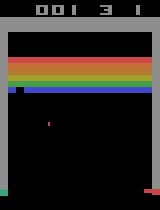
\includegraphics[]{breakout.jpg}
            \caption{\textit{Breakout}, do videogame \textit{Atari 2600}.}
            % https://gym.openai.com/videos/2019-10-21--mqt8Qj1mwo/Breakout-v0/poster.jpg
            \label{fig:breakout}
        \end{figure}

        Consegui implementar um algoritmo tal que é verificável que ele está "aprendendo"\ e que
        atinge pontuações legais para um programa de computador. Não atingi o estado da arte dessa
        implementação (estado este que é realmente impressionante),
        pois me deparei com algumas dificuldades,
        como escolhas dos hiperparâmetros e otimizações do tempo de execução.
        Tive acesso a uma máquina virtual mais pontente para
        o treinamento das redes neurais visando diminuir o tempo de execução
        do código.
        
        Aprendi muito sobre ferramentas para implementação
        de algoritmos de redes neurais, como a biblioteca \textit{TensorFlow},
        o painel de avaliação \textit{TensorBoard} e o \textit{profiler} de
        algoritmos \textit{TensorFlow Profiler}. Realizei, no final de maio,
        uma apresentação
        % https://github.com/lucasresck/deep-reinforcement-learning/blob/master/presentations/introduction_to_tensorflow/introduction_to_tensorflow.ipynb
        sobre a biblioteca \textit{TensorFlow}, para o grupo de pesquisa.

    \section{Visualização na Web}

        Recentemente, no início de julho, iniciei estudos sobre visualização
        na web, utilizando a biblioteca \textit{D3} para \textit{JavaScript} e 
        \textit{notebooks} interativos da \textit{Observable}. Eles permitem
        implementar e executar códigos \textit{JavaScript} e \textit{HTML}
        para visualização de dados interativa no navegador.

    \section{Futuras extensões}

        É esperado que o projeto continue. Uma possível extensão dos estudos
        em visualização na web é realizar visualizações do algoritmo de \textit{Deep Q-Learning}
        implementado anteriormente, gerando \textit{insights} do tipo \textit{"como o algoritmo está aprendendo"}\
        ou \textit{"como a rede neural reage a determinada situação do jogo"}.

    \bibliographystyle{plain}
    \bibliography{references}
\end{document}
